% !TEX root = FDS_Technical_Reference_Guide.tex

\typeout{new file: Combustion_Chapter.tex}

\chapter{Combustion (Chemically Reacting Flows)}
\label{chapter:combustion}

\label{combustionsection}
The combustion model determines the mean chemical mass production rate of species $\alpha$ per unit volume, $\dot{m}^{\prime\prime\prime}_{\alpha}$, in the species transport equation, Eq.~(\ref{species}).  In general, $\dot{m}^{\prime\prime\prime}_{\alpha}$ requires a closure model because the flame thickness is on the order of one millimeter while the grid spacing is typically on the order of tens of centimeters.  This chapter describes a turbulent batch reactor model for $\dot{m}^{\prime\prime\prime}_{\alpha}$ capable of handling a range of mixing conditions and chemical kinetics.  In the non-premixed, fast chemistry limit, which is valid for the vast majority of FDS applications, the reactor model reduces to a simple ``mixed is burnt'' approximation called the Eddy Dissipation Concept (EDC) \cite{Magnussen:1,Poinsot:TNC}.

The combustion model also determines the heat release rate per unit volume, $\dot{q}^{\prime\prime\prime}$, which is a quantity of fundamental importance in fire physics and typically the largest contribution to the velocity divergence, Eq.~(\ref{eqn_fdsD1}).  Once $\dot{m}^{\prime\prime\prime}_{\alpha}$ has been determined, the heat release rate follows by summing the mass production rates for each species times their respective heats of formation.  Details are discussed below in Section \ref{sec:hrr}.

Before discussing the combustion model, we first discuss of our \emph{lumped species} approach (Section~\ref{sec:lumpedspecies}), which reduces the computational burden of the full chemical system by combining species into groups that transport and react together.  In other words, we reduce the number of transport equations we need to solve, which significantly increases the speed of the computation.

In Section~\ref{sec:batchreactormodel}, we begin the discussion of our generalized combustion model which is designed to handle both fast and slow chemistry and a range of mixing conditions.  For fire, this method holds the promise for improved prediction of carbon monoxide and soot. Each computational cell is treated as a partially-stirred batch reactor with a characteristic mixing time.  Once reactants are mixed, the available reaction mechanisms range from infinitely fast chemistry to Arrhenius rate laws and reversible reactions. Our basic mixing-controlled, fast chemistry combustion model is presented in Section~\ref{sec:fastchemistry}. Section~\ref{extinction} discusses several options for modeling extinction.

\section{Lumped Species Approach}
\label{sec:lumpedspecies}

In the typical FDS problem the primitive species are lumped into reacting groups and we consider the simple reaction
\begin{equation}\label{eq:simple}
\mathrm{Fuel + Air \rightarrow Products}
\end{equation}
We refer to the Fuel, Air, and Products in Eq.~(\ref{eq:simple}) as \emph{lumped species}.  The lumped species approach is a simplified reaction progress variable approach~\cite{fox2003} in which all the progress variables are mass fractions. This avoids any complications related to boundedness and ill-defined initial and boundary conditions.

\subsection{Relationship between Lumped and Primitive Species}

In a simple hydrocarbon reaction, the reactants are the fuel, oxygen, and nitrogen and the products are carbon dioxide, water vapor, and nitrogen. For methane, the primitive species mass fractions are given by the composition vector
\begin{equation}\label{eq:prim_vector}
\mathbf{Y} = [Y_{\mathrm{CH}_4}\, \, Y_{\mathrm{O}_2}\, \, Y_{\mathrm{N}_2}\, \, Y_{\mathrm{CO}_2}\, \, Y_{\mathrm{H}_2\mathrm{O}}]^T
\end{equation}
Lumped species are groups of primitive species which only exist in the flow in certain proportions. For example, Air can be assumed to be a lumped species composed of 21~\% O$_2$, 79~\% N$_2$ by volume, plus trace amounts of water vapor and carbon dioxide. The key assumption made in lumping primitive species is that the new species groups transport (implying equal diffusivities) and react together.

In terms of primitive species, a one-step methane reaction may be written as
\begin{equation}\label{eq:lumped_methane}
\mbox{CH}_4 + 2\, \mbox{O}_2+7.52\,\mbox{N}_2 \rightarrow \mbox{CO}_2+2\,\mbox{H}_2\mbox{O}+7.52\,\mbox{N}_2
\end{equation}
This is equivalent to
\begin{equation}\label{eq:lumped_expand}
\mathrm{9.52\underbrace{(0.21\,\mbox{O}_2+.79\,\mbox{N}_2)}_\text{Air, $Z_1$} + \underbrace{ \mbox{CH}_4}_\text{Fuel,~$Z_2$} \rightarrow 10.52\underbrace{(0.095\,\mbox{CO}_2+0.19\,\mbox{H}_2\mbox{O}+0.715\,\mbox{N}_2)}_\text{Products,~$Z_3$}}
\end{equation}
where 9.52~moles of Air react with 1~mole of Fuel to produce 10.52~moles of Products. Notice that the primitive species have been grouped by volume fraction into lumped species and the lumped species stoichiometric coefficients are the sum of the primitive species coefficients from Eq.~(\ref{eq:lumped_methane}). Note that 9.52 $\times$ 0.21 is only approximately equal to 2. In practice the atom balance requires machine precision. To alleviate this issue, FDS internally normalizes the lumped species volume fractions and makes any necessary adjustments to the specified lumped stoichiometric coefficients. The lumped species mass fractions are denoted $Z_i$, $i=1,...,N_Z$, where $N_Z$ is the number of tracked species. The first tracked species, $Z_1$, is typically the background species, Air.

The linear transformation from lumped species to primitive species is given by
\begin{equation}\label{eq:transform}
\textbf{Y}=A\textbf{Z}
\end{equation}
where $A$ is the transformation matrix ($N_{y}$ rows $\times$ $N_{z}$ columns).  Each column of $A$ represents a different lumped species.  The elements of $A$ are the mass fractions for each primitive species in a given lumped species:
\begin{equation}\label{eq:A_def}
a_{\alpha\,i} = \frac{\upsilon_{\alpha\,i}W_{\alpha}}{\displaystyle \sum_{\beta}\upsilon_{\beta i}W_{\beta}}
\end{equation}
where $\upsilon_{\alpha\,i}$ are the volume fractions of primitive species $\alpha$ in lumped species $i$ and $W_\alpha$ are the molecular weights. If we want the primitive species in Eq.~(\ref{eq:lumped_expand}) and, as an example, say we have $\mathbf{Z} = [0.3 \,\,\, 0.2 \,\,\, 0.5]^T$, we can transform from lumped species to primitive species via

\begin{equation}\label{eq:transform_to_primitive}
\mathbf{Y}=\left[\begin{array}{c}
       Y_{\mathrm{O}_2} \\
       Y_{\mathrm{N}_2} \\
       Y_{\mathrm{CH}_4} \\
       Y_{\mathrm{CO}_2} \\
       Y_{\mathrm{H}_2\mathrm{O}} \\
     \end{array}\right]
     =\left[\begin{array}{ccc}
     0.2330 & 0 & 0 \\
     0.7670 & 0 & 0.7248 \\
     0 & 1 & 0 \\
     0 & 0 & 0.1514 \\
     0 & 0 & 0.1238 \\
     \end{array}\right]
     \left[\begin{array}{c}
     0.3 \\
     0.2 \\
     0.5 \\
     \end{array}\right]
     =\left[\begin{array}{c}
     0.0699\\
     0.5925\\
     0.2000\\
     0.0757\\
     0.0619\\
     \end{array}\right]
\end{equation}
To transform back to lumped species from primitive species we can use:
\begin{equation}\label{eq:transform_back}
\textbf{Z}=B\textbf{Y} \quad ; \quad B=(A^TA)^{-1}A^T
\end{equation}
provided $A$ has full rank and $\mathbf{Y}$ is realizable (i.e., the forward transformation is also possible).

\subsection{Default Hydrocarbon Combustion Chemistry}
\label{sec:simplechemistry}

The default reaction equation in FDS, known as ``simple chemistry,'' is defined as follows:
\begin{multline}\label{eq:full_lump}
\nu_{1}\underbrace{(\upsilon_{\mathrm{O}_{2},1} \, \mathrm{O}_2 +\upsilon_{\mathrm{N}_{2},1} \, \mathrm{N}_2 + \upsilon_{\mathrm{H}_{2} \, \mathrm{O},1} \, \mathrm{H}_2 \, \mathrm{O}+\upsilon_{\mathrm{CO}_{2},1} \, \mathrm{CO}_2)}_\text{Background,~$Z_1$} \; + \; \nu_{2} \, \underbrace{\mbox{C}_m\mbox{H}_n\mbox{O}_a\mbox{N}_b}_\text{Fuel,~$Z_2$} \quad \longrightarrow \\
\nu_{3}\underbrace{(\upsilon_{\mathrm{CO}_{2},3} \, \mathrm{CO}_2 + \upsilon_{\mathrm{H}_{2} \, \mathrm{O},3} \, \mathrm{H}_2 \, \mathrm{O} + \upsilon_{\mathrm{N}_{2},3} \, \mathrm{N}_2+\upsilon_{\mathrm{CO},3} \, \mathrm{CO} + \upsilon_{\mathrm{S},3} \, \mathrm{Soot})}_\text{Products,~$Z_3$}
\end{multline}
Here, the volume fraction of primitive species $\alpha$ in lumped species $i$ is denoted by $\upsilon_{\alpha\,i}$ and the stoichiometric coefficients for the lumped species $i$ are denoted by $\nu_{i}$.

Carbon monoxide and soot yields are zero by default. The user can specify the CO and soot yields ($y_{\mathrm{CO}}$ and $y_{\mathrm{S}}$ respectively). The CO yield, and similarly for soot, is the mass of CO produced per mass of fuel reacted:
\begin{equation}\label{eq:y_co}
y_\mathrm{CO} = \frac{\mbox{mass CO in Products}}{\mbox{mass of Fuel reacted}}
\end{equation}
In this reaction system, Air (Background) is lumped species 1, Fuel is lumped species 2, and Products is lumped species 3. To find the stoichiometric coefficients of CO and soot within the products lumped species, FDS uses
\begin{align}\label{eq:yields}
\nu_{2}\upsilon_{\mathrm{CO},2}&=-\nu_{1}\frac{W_1}{W_{\mathrm{CO}}}y_{\mathrm{CO}} \\
\nu_{2}\upsilon_{\mathrm{S},2}&=-\nu_{1}\frac{W_1}{W_{\mathrm{S}}}y_{\mathrm{S}}
\end{align}
The remaining coefficients come from an atom balance.

\paragraph{Example} Consider a methane--air reaction where methane has a specified CO yield of $y_{\mathrm{CO}}=0.1$ and a Soot yield of $y_{\mathrm{S}}=0.01$. The default FDS reaction system lumps these species into Products. Note that, by default, Air is primarily composed of oxygen and nitrogen but includes trace amounts of carbon dioxide and water vapor. For this reaction the transformation matrix, $A$, is

\begin{center}
\begin{tabular}{c c c c }
                   & Air & Fuel & Products \\ \hline
{CH$_4$}           & 0.000000 & 1.000000 & 0.000000 \\
{N$_2$}            & 0.763017 & 0.000000 & 0.720373 \\
{O$_2$}            & 0.231163 & 0.000000 & 0.000000 \\
{CO$_2$}           & 0.000592 & 0.000000 & 0.143067 \\
{CO}               & 0.000000 & 0.000000 & 0.005589 \\
{H$_2$O}           & 0.005228 & 0.000000 & 0.130412 \\
{C}                & 0.000000 & 0.000000 & 0.000559 \\
\end{tabular}
\end{center}

\noindent The preceding table shows that the addition of carbon monoxide and soot increases the number of primitive species in the reaction from five to seven. The number of lumped species, however, remains at three---the composition of Products has changed to include to the two additional species.  Note that FDS prints the $A$ matrix in the {\ct CHID.out} file so that the user can double check the reaction system.


\clearpage

\section{Turbulent Combustion}
\label{sec:batchreactormodel}

Modeling chemical reactions in turbulent flow is mathematically challenging because the length and time scales associated with the reactions may be orders of magnitude below what can be spatially and temporally resolved by the simulation.  When the fuel and oxidizer are initially unmixed (diffusion flame) and the kinetics are fast compared with mixing, the simple Eddy Dissipation Concept (EDC) model \cite{Magnussen:1,Poinsot:TNC} is sufficient.  However, for more complex reactions---such as carbon monoxide and soot formation---where reaction and mixing time scales may overlap, we require a more generalized approach.

To this end, we have developed a simple mixing environment method to close the mean chemical source term, $\dot{m}^{\prime\prime\prime}_{\alpha}$, in Eq.~(\ref{species}).  For pure diffusion flames our method is similar to EDC, but the method is not limited to diffusion flames.  Each computational cell is thought of as a {\em turbulent batch reactor}. At the start of a time step, each cell has an initial concentration of species (reactants, products, inerts) that exist with some degree of mixing. Generally, the rate of mixing is dominated by turbulence. The mixing time, $\tau_{\rm mix}$, is discussed in Section~\ref{sec:reac_time_scale}. The mixing/reacting evolution equation and its numerical solution are described in Sections~\ref{sec:subgrid_evironment}~and~\ref{sec:reac_time_integration}. Once mixed, species can react based on specified kinetic parameters---reactions may be infinitely fast (Section~\ref{sec:fastchemistry}) or governed by an Arrhenius rate law (Section~\ref{Reaction_Rate_Model}).


\subsection{Reaction Time Scale Model}
\label{sec:reac_time_scale}

In this section we provide an expression for the mixing time based on the local state of the flow field.  The basic idea behind the model we propose here is to consider the three physical processes of diffusion, subgrid-scale (SGS) advection, and buoyant acceleration and to take the fastest of these processes (locally) as the controlling flow time scale~\cite{McDermott:2011}.

It is important to consider the behavior of an SGS model as the LES filter width (cell size) varies. The mixing times for diffusion, SGS advection, and buoyant acceleration scale differently with filter width and if we look to the limits of the filter scales an interesting picture emerges.  Referring to Fig.~\ref{fig_reaction_time_scale}, let us move from left to right along the horizontal axis following the thick black line which represents our time scale model for a hypothetical flow condition.

First, notice that the reaction time scale must be greater than or equal to the chemical time scale, $\tau_{\rm chem}$, which is of the order of the traversal time of the flame thickness, $\tau_{\rm chem} \sim \delta/s_{\rm L}$, where $\delta=D_{\rm F}/s_{\rm L}$, $D_{\rm F}$ is the diffusivity of the fuel, and $s_{\rm L}$ is the flame speed. At a slightly larger scale, we expect the mixing time to vary as the square of the filter width because the mixing is controlled by molecular diffusion.  In this regime, denoted $\tau_{\rm d}$, the numerical solution is a DNS and this scaling law is valid while $\Delta$ is less than the Kolmogorov scale, $\eta$, the length scale of the smallest turbulent eddies (for this discussion we assume the Schmidt number (Sc) is of order unity). For a sufficiently high Reynolds number flow (such that an inertial subrange exists), as the filter width increases beyond the Kolmogorov scale we encounter a regime, marked $\tau_{\rm u}$, where turbulent advection controls the rate of mixing and the mixing time varies as the two-thirds power of the filter width \cite{Pope:2000}.  This is the regime where most LES submodels are valid (It is important to appreciate that fire differs from turbulent combustion in that the assumption of locally high Re is frequently invalid).

Now, let us imagine what should happen to the mixing time as the filter width increases beyond the inertial subrange to a length scale larger than the height of the flame itself (actually a possibility in wildfire modeling). We would \emph{not} expect the inertial range scaling to continue up through the so-called ``energy-containing'' range of turbulent length scales.  Rather, for fires we expect buoyant acceleration to control the mixing at these relatively coarse scales.  A time scale based on a constant acceleration goes as the square root of the filter width, as shown by the regime marked $\tau_{\rm g}$ in the diagram.  This shift in scaling may appear minor given the log-log nature of the plot, but the effect of the acceleration-based time scale is indeed significant for large cell sizes.  Finally, note that the flame height presents a limit to the reaction time scale, here denoted $\tau_{\rm flame}$, since all fuel must be consumed within a single cell.

\begin{figure}
\centering
\includegraphics[width=4.5in]{FIGURES/reaction_time_scale}
\vskip-.2cm
\caption{Reaction time scale model.}
\label{fig_reaction_time_scale}
\end{figure}

Of course, the relative importance of the physical processes will depend on the flow.  For example, if gravity is weak, the $\tau_{\rm g}$ line shifts up and may not affect the reaction time before the flame time scale is reached.  If the flow is highly turbulent, the inertial range scaling may be more dominant, which would be indicated by a lowering of the $\tau_{\rm u}$ line.  Or, for highly turbulent jet flames $\tau_{\rm flame}$ may be reached before the acceleration time scale has any effect.  Perhaps more typical for low strain fires, if an inertial subrange does not exist (if the Reynolds number is too low relative to the Froude number), then the $\tau_{\rm u}$ line in Fig.~\ref{fig_reaction_time_scale} moves up out of the picture and we are left with diffusion and buoyancy to control the mixing.

The bold solid line in Fig.~\ref{fig_reaction_time_scale} is mathematically represented by
\begin{equation}
\label{eqn_tau_mix}
\tau_{\rm mix} = \max(\tau_{\rm chem},\min(\tau_{\rm d},\tau_{\rm u},\tau_{\rm g},\tau_{\rm flame}))
\end{equation}
The mathematical details of the submodels are as follows:
\begin{align}
\label{eq:tau_diff} \tau_{\rm d} &= \frac{\Delta^2}{D_{\si{F}}} \\
\label{eq:tau_sgs}  \tau_{\rm u} &= \frac{C_u \,\Delta}{\sqrt{(2/3)k_{\rm sgs}}} \\
\label{eqn_tau_grav}\tau_{\rm g} &= \sqrt{ 2\Delta/g }
\end{align}
where $D_{\si{F}}$ is the diffusivity of the fuel species. Note that $k_{\rm sgs}$ is the unclosed subgrid kinetic energy per unit mass which by default is taken from the model for the turbulent viscosity (see Section~\ref{section:turbulent_viscosity}, Eq.~(\ref{Deardorff_LES})).  The advective time scale constant is calibrated to match the Heskestad flame height correlation \cite{FDS_Validation_Guide} and is set to $C_u = 0.4$. The acceleration time scale $\tau_{\rm g}$ is the time required to travel a distance $\Delta$ starting from rest under a constant acceleration, $g=\SI{9.81}{m/s^2}$.



\subsection{Time Integration for Mixing and Reaction}
\label{sec:subgrid_evironment}

Let the cell mean mass fraction of species $\alpha$ be denoted as $\widetilde{Y}_\alpha(t)$. Assume that any small parcel of gas within the cell exists in one of two states: completely unmixed or completely mixed.  Let $\hat{Y}_\alpha(t)$ denote the mass fraction of species $\alpha$ in the mixed reactor zone, initially equal to the cell mean, $\hat{Y}_\alpha(0) = \widetilde{Y}_{\alpha}^0 \equiv \widetilde{Y}_{\alpha}(0)$. For convenience, we define $\zeta(t)$ as the unmixed fraction of mass within the cell. As shown in Appendix~\ref{app:unmixed_fraction}, the unmixed fraction evolves by the following simple ordinary differential equation (ODE):
\begin{equation}
\label{eq:zeta}
\frac{\d \zeta}{\d t}=-\frac{\zeta}{\tau_{\rm mix}}
\end{equation}
with the solution
\begin{equation}
\label{eq:zeta_soln}
\zeta(t) = \zeta_0 \,{\rm e}^{-t/\tau_{\rm mix}}
\end{equation}
The initial condition, $\zeta_0$, may be specified, modeled algebraically, or taken from the update of a passive scalar transport equation.  Currently, FDS takes $\zeta_0=1$ as default, an appropriate assumption for a turbulent diffusion flame.

At any point in time, the composition of the computational cell may be determined by combining the unmixed and mixed portions:
\begin{equation}
\label{eq:final_comp}
\widetilde{Y}_{\alpha}(t)= \zeta(t) \, \widetilde{Y}_{\alpha}^0 + (1-\zeta(t)) \, \hat{Y}_{\alpha}(t)
\end{equation}
Differentiating (\ref{eq:final_comp}) in time and using (\ref{eq:zeta}) we see that our model for the chemical source term needed in (\ref{species}) is given by
\begin{equation}
\label{mass_prod_rate}
\dot{m}^{\prime\prime\prime}_{\alpha} = \rho \frac{\mbox{d}\widetilde{Y}_{\alpha}}{\mbox{d}t}
= \rho \left[ \frac{\zeta}{\tau_{\rm{mix}}} (\hat{Y}_\alpha - \widetilde{Y}_{\alpha}^0)  + (1-\zeta) \frac{\mbox{d}\hat{Y}_\alpha}{\mbox{d}t} \right]
\end{equation}
Note that the unmixed fraction is comparable to the \emph{complement} of the fraction of ``reacting fine structures'' in other EDC formulations \cite{Chen:1,Panjwani:2010}, but in our model this fraction evolves in time.  A comparison between our model and that of Panjwani et al.~\cite{Panjwani:2010} is developed further in Appendix~\ref{app:eddy_dissipation_concept}. An alternate derivation of (\ref{eq:final_comp}) and (\ref{mass_prod_rate}) in terms of moments of the transport equation for the PDF is given in Appendix~\ref{app:pdf_transport}.  This derivation highlights that the implicit mixing model is a variant of the {\em interaction by exchange with the mean} or IEM model~\cite{Dopazo:1974}, which we refer to as the {\em interaction by exchange with the mixed mean} or IEMM.

Rather than work with the evolution equation (\ref{mass_prod_rate}) for the cell mean mass fraction, $\widetilde{Y}_\alpha(t)$, it is more convenient to work with an analogous equation for the mass fraction within the mixed reactor zone, $\hat{Y}_\alpha(t)$. This equivalent evolution equation is derived as follows. It is assumed that the total mass within the grid cell is constant over a time step. The composition in the mixed reactor zone changes by two processes: mixing (mass is transferred from the unmixed zone to the mixed zone) and chemical reaction. We denote this mass by $\rho V_{\rm c}$, where $\rho$ is the initial cell mass density and $V_{\rm c}$ is the cell volume.  The unmixed mass is denoted $U(t)$ and the mixed mass is denoted $M(t)$.  Given (\ref{eq:zeta_soln}), the following equations describe the cell mass evolution:
\begin{align}
\label{eq:mixunmix_1} \rho V_{\rm c} &= U(t) + M(t) \\[0.1in]
\label{eq:mixunmix_2} U(t) &= \zeta(t)\,\rho V_{\rm c} \\[0.1in]
\label{eq:mixunmix_3} M(t) &= (1-\zeta(t))\,\rho V_{\rm c}
\end{align}
Within the mixed reactor zone, let $\hat{m}_\alpha(t)$ denote the mass of species $\alpha$.  The mass fraction of $\alpha$ in the mixed zone may then be written as
\begin{equation}
\label{eq:mass_fraction_mixed}
\hat{Y}_{\alpha}(t)\equiv\frac{\hat{m}_{\alpha}(t)}{M(t)}
\end{equation}
This concentration is important because Arrhenius rate laws are based on the mixed composition only. The ODE governing the mixed species mass is
\begin{align}
\label{eq:mixmass}
\frac{\d \hat{m}_{\alpha}}{\d t} &= \hat{Y}_\alpha \frac{\d M}{\d t} + M \frac{\d \hat{Y}_\alpha}{\d t} \notag\\[0.1in]
&= - \widetilde{Y}_{\alpha}^0 \frac{\d U}{\d t} + M \frac{\d \hat{Y}_\alpha}{\d t} \notag\\[0.1in]
&= \rho V_{\rm c} \left[ \frac{\zeta \, \widetilde{Y}_{\alpha}^0 }{\tau_{\rm mix}} + (1-\zeta) \frac{\d \hat{Y}_\alpha}{\d t} \right]
\end{align}
The first term  on the RHS accounts for mixing.  The second term represents chemical kinetics. Note that in the second step we have utilized the fact that the unmixed composition remains constant (at the initial cell mean) throughout the time step. The third step follows from (\ref{eq:zeta}), (\ref{eq:mixunmix_2}), and (\ref{eq:mixunmix_3}).

\subsection{Numerical Solution via Time-Splitting}
\label{sec:reac_time_integration}

In this section, we discuss the numerical solution of (\ref{eq:mixmass}). Let $\Delta t^k$ represent the $k$th sub-time step in the integration (less than or equal to the LES time step $\delta t$); $t^k=0$ at the start of the reactor integration.  The integration is time split such that \emph{mixing is done first, followed by reaction}. A simple explicit update of (\ref{eq:mixmass}) over the sub-time interval $t^k$ to $t^k + \Delta t^k$ is given by
\begin{align}
\label{eq:dmdt_1} \hat{m}_\alpha^* &= \hat{m}_{\alpha}(t^k) - [ \zeta(t^k+\Delta t^k) - \zeta(t^k) ] \, \widetilde{Y}_{\alpha}^0 \, \rho V_{\rm c} \\[0.1in]
\label{eq:ystar}  \hat{Y}_\alpha^* &= \hat{m}_\alpha^*/M^* \\[0.1in]
\label{eq:dmdt_2} \hat{Y}_\alpha(t^k + \Delta t^k) &= \hat{Y}_\alpha^* + \Delta \hat{Y}_\alpha^*
\end{align}
The superscript $^*$ indicates a post-mixing value.  The first step, (\ref{eq:dmdt_1}), is an analytical solution for the mixing step (first term in (\ref{eq:mixmass})), obtained using (\ref{eq:zeta_soln}).  The mixing time scale $\tau_{\rm mix}$, needed in (\ref{eq:zeta_soln}), is computed once per LES time step using (\ref{eqn_tau_mix}) and held constant during the reactor integration. The mixed mass, $M^* = M(t^k + \Delta t^k)$, is evaluated at the end of the subinterval using (\ref{eq:mixunmix_3}). For fast chemistry, we take only one sub-step ($\Delta t^{k=1} = \delta t$). At the end of the time integration, the mixed zone composition, $\hat{Y}_\alpha(\delta t)$, is combined with the unmixed mass to obtain the final cell composition.

The method to determine $\Delta \hat{Y}_\alpha^*$ (the change in mass fraction of $\alpha$ due to chemical reaction) in (\ref{eq:dmdt_2}) depends on the complexity of the reaction system. In the next section, we first discuss the simplest case of infinitely fast chemistry.  Then we discuss finite-rate chemistry.



\subsection{Infinitely Fast Chemistry}
\label{sec:fastchemistry}

\subsubsection{Single Reaction}

For a single reaction, the change in fuel is based on the limiting reactant \cite{Poinsot:TNC}:
\begin{equation}\label{eq:stoich_fuel_single}
\Delta \hat{Y}_{\rm F} = -\min \left( \hat{Y}_{\rm F}, \hat{Y}_{\alpha} \,\frac{\nu_{\rm F}\,W_{\rm F}}{\nu_{\alpha}\,W_{\alpha}}\right) \quad ; \quad \mbox{for all reactants, $\alpha$}
\end{equation}
The minimum is taken in Eq.~(\ref{eq:stoich_fuel_single}) to ensure that the reactant species mass fractions remain realizable.

This approach is used for the vast majority of large-scale fire applications---the so-called ``mixed is burnt'' assumption, where the mean chemical source term for the Fuel, F, is modeled using the Eddy Dissipation Concept (EDC) of Magnussen and Hjertager~\cite{Magnussen:1,Poinsot:TNC}:
\begin{equation}
\label{eq:edc}
\dot{m}_{\si{F}}^{\prime\prime\prime} = -\rho \frac{\min(Y_{\si{F}}, Y_{\si{A}}/s)}{\tau_{\rm mix}}
\end{equation}
Here, $Y_{\si{F}}$ and $Y_{\si{A}}$ are the cell mean mass fractions of Fuel and Air, respectively, and $s$ is the mass stoichiometric coefficient for Air.

\subsubsection{Multiple Reactions}
For multiple reactions with infinitely fast chemistry, the reaction rate is treated as a second-order (assuming two reactants) Arrhenius reaction with zero activation energy.  The Arrhenius constant is set to a large value.  Further discussion of the time integration for these cases is given in Appendix \ref{chemistry_integration}.


\subsection{Finite-Rate Chemistry (Arrhenius Reaction)}
\label{Reaction_Rate_Model}

Consider a simple one-step forward reaction:
\begin{equation}\label{eq:generic_1step}
a\mathrm{A} + b\mathrm{B} \rightarrow c\mathrm{C} + d\mathrm{D}
\end{equation}
The rate expression for species A with a mixed zone concentration of $C_{\mbox{\scriptsize A}}$ in \si{mol/cm^3} and rate constant $k$ is
\begin{equation}\label{eq:generic_rate}
\frac{\d C_{\mbox{\scriptsize A}}}{\d t}= -k\; C_{\mbox{\scriptsize A}}^{\,a}\; C_{\mbox{\scriptsize B}}^{\,b}
\end{equation}
Consider a set of $N_r$ reactions with fuel F. The reaction rate (\si{mol/(cm^3.s)}) for F in the $i$th reaction is
\begin{equation}\label{eq:rate_f}
r_{\si{F},i}= -k_{i}\; \prod C_{\alpha}^{\,a_{\alpha,i}}
\end{equation}
For the $i$th Arrhenius reaction, the rate constant, $k_i$, depends on the temperature, $T$, the temperature exponent, $n_i$, the pre-exponential factor, $A_i$, and the activation energy, $E_i$:
\begin{equation}\label{eq:rate_cons}
k_i = A_i\;T^{n_i}\;\mathrm{e}^{-E_{a,i}/RT}
\end{equation}
Note that the units of $E_a$ are J/mol and units of $A$ are ((\si{mol/cm^3})$^{1-\sum a_{\alpha}}$)/s.  Note that $\sum a_{\alpha}$ is the \emph{order} of the reaction.  The units of $A$ take the appropriate form to ensure the units of Eq.~(\ref{eq:rate_f}) are \si{mol/(cm^3.s)}.

The reaction rate for species $\alpha$ of the $i$th reaction is based on the ratio of stoichiometric coefficients:
\begin{equation}\label{eq:rate_a}
r_{\alpha,i}= \left(\frac{\nu_{\alpha,i}}{\nu_{F,i}}\right)\,r_{\si{F},i}
\end{equation}
The change in concentration for species $\alpha$ within the mixed reactor zone is then:
\begin{equation}\label{rate_expression}
\frac{\d C_{\alpha}}{\d t} = \sum_{i} r_{\alpha,i}
\end{equation}
FDS only transports lumped species and only lumped species can be consumed or created.  Note, however, that any of the primitive species may participate in a reaction rate law.

It is more convenient for FDS to work in terms of mass fractions, $Y_{\alpha}$.  The concentrations (\si{mol-$\alpha$/cm^3}) and mass fractions (kg-$\alpha$/kg) are related by $C_{\alpha}=Y_{\alpha} \rho/(W_{\alpha} \times 1000)$, where the density, $\rho$, has units of \si{kg/m^3}.
To simplify the calculations within FDS, density and molecular weight are pulled out of the product concentrations on the right hand side of Eq.~(\ref{eq:rate_f}) and combined with the other constants to form $A^{\prime}$:
\begin{equation}\label{eq:aprime}
A^{\prime}_{i} = A_{i} \, \bigg( \prod \, [W_{\alpha} \times 1000]^{\,-a_{\alpha,i}} \bigg) \times \left(\frac{1 \; \si{kmol}}{10^3 \; \si{mol}}\right) \times \left(\frac{10^6 \; \si{cm^3}}{1 \; \si{m^3}}\right) \times W_{\,\si{F}}
\end{equation}
Using $A_i^{\prime}$, the reaction rate in mass units becomes
\begin{equation}\label{eq:finite_rate_fin}
r^{\prime}_{\si{F},i} = -A_i^{\prime}\;\rho^{\sum a_{\alpha,i}}\;T^{n_i}\;\mathrm{e}^{-E_i/RT}\;\prod Y_{\alpha}^{\,a_{\alpha,i}} \quad [=] \quad \left(\frac{\si{kg \; F}}{\si{m^3.s}}\right)
\end{equation}
The mass rate of reaction per unit volume for species $\alpha$ in the $i$th reaction is
\begin{equation}\label{eq:rate_a_y}
r^{\prime}_{\alpha,i}= \left(\frac{\nu_{\alpha,i}\,W_{\alpha}}{\nu_{\si{F},i}\,W_{\,\si{F}}}\right)\,r^{\prime}_{\si{F},i} \quad [=] \quad \left(\frac{\si{kg \; \alpha}}{\si{m^3.s}}\right)
\end{equation}
Last, the rate of change in composition for species $\alpha$ in the mixed reactor zone becomes
\begin{equation}\label{rate_expression_y}
\frac{\d \hat{Y}_{\alpha}}{\d t} = \frac{1}{\rho}\sum_{i} r^{\prime}_{\alpha,i} \quad [=] \quad \left(\frac{\si{kg \; \alpha}}{\si{kg.s}}\right)
\end{equation}
See Appendix~\ref{chemistry_integration} for a discussion on the algorithm used to ensure species remain bounded.

\subsubsection{Third Body Reactions}

At low pressures, it is common to see so-called \emph{third body} reactions.  These reactions require the presence of some other molecule, M, for heat dissipation \cite{Turns:1996}.  The reaction scheme is usually written as
\begin{equation}\label{eq:third_body}
\mathrm{A} + \mathrm{B} + \mathrm{M} \rightarrow \mathrm{C} + \mathrm{M}
\end{equation}
The Arrhenius rate law has a first-order dependence on the concentration of M.  Since M may be \emph{any} other molecule, we take $C_{\si{M}} = \bar{p}/(R T) = \rho/(\overline{W} \times 1000) \;[=]\;\si{mol/cm^3}$.

\subsubsection{Time Integration for Finite-Rate Chemistry}

For reactions other than single step, mixing controlled chemistry, a fourth-order explicit integrator with error control is used. The time integration follows the procedure outlined in Eqs.~(\ref{eq:dmdt_1}) and (\ref{eq:dmdt_2}), but multiple subiterations are generally needed and the change in composition over the subinterval in the mixed reactor zone, $\Delta \hat{Y}_\alpha^*$, is usually obtained by integrating an Arrhenius rate law (we say ``usually'' because a combination of fast and finite-rate chemistry is permissible). More detail on the numerical methods of the integrator, including a method to combat stiff chemistry, can be found in Appendix~\ref{chemistry_integration}.


\subsection{Heat Release Rate}
\label{sec:hrr}

At the end of the LES/DNS time step, $\delta t$, the mixed reactor zone mass fraction of species alpha is computed using the change in fuel concentration for each of the $N_{\rm r}$ reactions:
\begin{equation}\label{eq:change_alpha}
\hat{Y}_\alpha(\delta t) = \widetilde{Y}_\alpha^0 + \sum_{i=1}^{N_{\rm r}} \,\left(\frac{\nu_{\alpha,i} \,W_{\alpha}}{\nu_{{\rm F},i} \,W_{{\rm F},i}}\right)\Delta \hat{Y}_{{\rm F},i}
\end{equation}
The new cell mean mass fraction is found be evaluating Eq.~(\ref{eq:final_comp}) at the end of the time step:
\begin{equation}
\label{eq:final_comp2}
\widetilde{Y}_{\alpha}(\delta t)= \zeta(\delta t) \, \widetilde{Y}_{\alpha}^0 + (1-\zeta(\delta t)) \, \hat{Y}_{\alpha}(\delta t)
\end{equation}
The heat release per unit volume is then found by summing the species mass production rates times the respective heats of formation:
\begin{equation}\label{eq:vol_heat_gen}
\dot{q}''' = \rho  \sum_{\alpha} \left( \widetilde{Y}_{\alpha}(\delta t)-\widetilde{Y}_{\alpha}^0 \right) \, \Delta h_{{\rm f},\alpha}^0
\end{equation}




\clearpage

\section{Extinction}
\label{extinction}

A limitation of the default mixing-controlled reaction model described above is that it assumes fuel and oxygen always react regardless of the local temperature, reactant concentration, or strain rate. For large-scale, well-ventilated fires, this approximation is usually sufficient. However, if a fire is in an under-ventilated compartment, or if a suppression agent like water mist or CO$_2$ is introduced, or if the strain between the fuel and oxidizing streams is high, burning may not occur.

FDS uses simple empirical rules---which ignore strain---to predict local extinction within a given grid cell based on resolved species concentrations and the mean cell temperature. There are two options for predicting extinction, both of which are based on the concept of a \emph{critical flame temperature}. The basic theory behind the critical flame temperature is described in Beyler's chapter of the SFPE Handbook~\cite{SFPE:Beyler} even though he never explicitly uses this term. In fact, it is mentioned only a few times in the Handbook, and each time it has a slightly different interpretation.


\subsection{Critical Flame Temperature}
\label{CFT}

A diffusion flame immersed in a vitiated atmosphere will extinguish before consuming all the available oxygen. The classic example of this behavior is a candle burning within an inverted jar.  With this picture in mind, consider a control volume characterized by a bulk temperature, $T$, a mass, $m$, and an oxygen mass fraction, $Y_\OTWO$.  Complete combustion of the oxygen within the control volume would release a quantity of energy given by:
\be
   Q = m \, Y_\OTWO \, \left( \frac{\Delta H}{r_\OTWO}  \right)  \label{bbb}
\ee
where $\Delta H/r_\OTWO$ has a relatively constant value of approximately 13100~kJ/kg for most fuels of interest in fire applications~\cite{Huggett:1}. Under adiabatic conditions, the energy released by the reaction of the available oxygen and the corresponding stoichiometric amount of fuel would increase the bulk temperature of the gases to $T_{\rm f}$:
\be
   Q = m \, \overline{c_p} \, (T_{\rm f} - T)  \label{eee}
\ee
The average specific heat of the gases can be calculated based on the composition of the combustion products as:
\be
   \overline{c_p} = \frac{1}{(T_{\rm f}-T)} \, \sum_\alpha \int_{T}^{T_{\rm f}} Y_\alpha \, c_{p,\alpha} (T') \, \d T'
\ee
Equating Eqs.~(\ref{bbb}) and (\ref{eee}) yields:
\be
   Y_\OTWO = \frac{ \overline{c_p} \, (T_{\rm f}-T) }{\Delta H/r_\OTWO} \label{YO2eq}
\ee
The critical flame temperature (CFT), as interpreted within FDS, is based on the {\em limiting oxygen index} (LOI), the oxygen volume fraction in the oxidant stream at the point of flame extinction. The adiabatic flame temperature corresponding to a stoichiometric mixture of fuel and oxygen at the LOI can be derived using Eq.~(\ref{YO2eq}):
\be
   T_{\OI} = T_\infty + Y_{\OI} \, \left( \frac{\Delta H/r_\OTWO}{\overline{c_p}} \right) \quad ; \quad  Y_{\OI} = \frac{X_{\OI} \, W_\OTWO}{X_{\OI} \, W_\OTWO + (1-X_{\OI}) \, W_\NTWO }
   \label{CFT_def}
\ee
Beyler's chapter of the SFPE Handbook~\cite{SFPE:Beyler} includes $X_{\OI}$ and $T_{\OI}$ for several common fuels. For other fuels, a default values are used. These values are given in the FDS User's Guide~\cite{FDS_Users_Guide}.

\subsection{Extinction Based Mainly on Oxygen Concentration}
\label{o2_based_model}

The first of two optional extinction models (referred to as {\ct 'EXTINCTION 1'} in the FDS input file) linearizes Eq.~(\ref{YO2eq}) to form a limiting oxygen concentration\footnote{The extinction model is written in terms of the oxygen {\em volume} fraction, $X_\OTWO$, because usually experimental results are reported as such. However, within the numerical algorithm, all values are converted into mass fraction, $Y_\OTWO$.} that is a piecewise-linear function of the cell bulk temperature, $T_{ijk}$ (see Fig.~\ref{extinction_1_sketch}):
\be
   X_{\OTWO,\lim}(T_{ijk}) = \left\{ \begin{array}{c@{\quad \quad}l} X_{\OI} \, \left( \frac{T_{\OI}-T_{ijk}}{T_{\OI}-T_\infty} \right) & T_{ijk}<T_{\rm fb} \\[.1in]  0 &  T_{ijk} \ge T_{\rm fb} \end{array} \right.  \label{extinction_model}
\ee
\begin{figure}
\centering
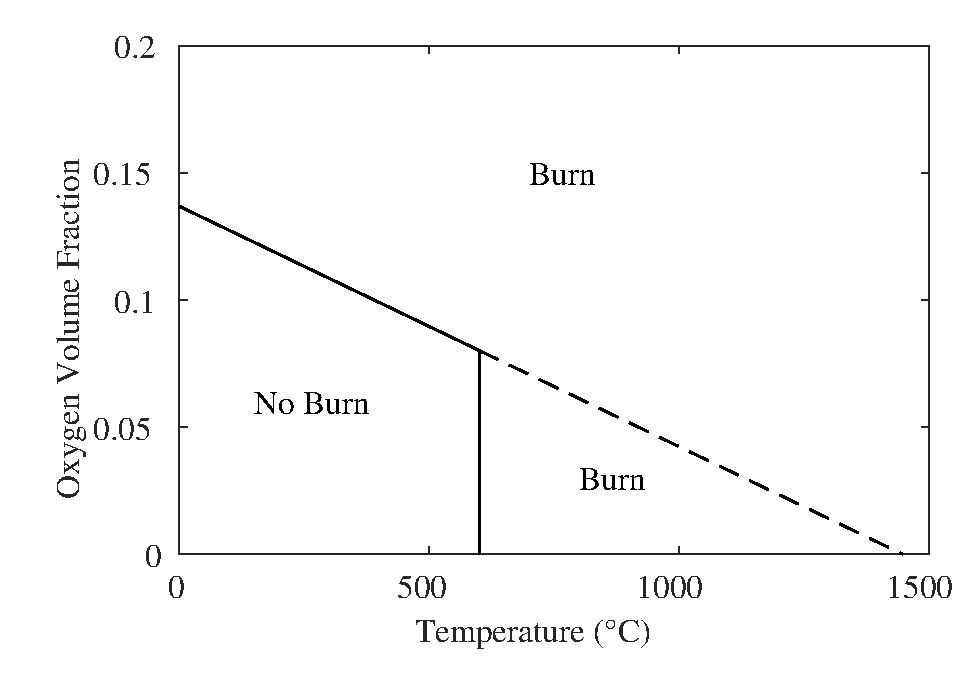
\includegraphics[width=4.5in]{FIGURES/extinction_1_sketch}
\vskip-.2cm
\caption{Extinction criteria for the {\ct 'EXTINCTION 1'} model.}
\label{extinction_1_sketch}
\end{figure}
If $X_{\OTWO,ijk}<X_{\OTWO,\lim}$, local extinction is assumed and $\dot{m}_\alpha'''=0$ and $\dot{q}'''=0$ for that grid cell at that time step. At an ambient temperature of 20~$^\circ$C, the default limiting oxygen volume fraction is 0.135.  This value is consistent with the measurements of Morehart et al.~\cite{Morehart:1991}, who measured the oxygen concentration near self-extinguishing flames. They found that flames self-extinguished at oxygen volume fractions of 12.4~\% to 14.3~\%. Note that their results are expressed as volume, not mass, fractions. Beyler's chapter in the SFPE Handbook references other researchers who measured oxygen concentrations at extinction ranging from 12~\% to 15~\%.

The {\ct 'EXTINCTION 1'} model is intended for relatively coarse fire simulations where the grid cell cannot resolve details of the flame structure or capture flame temperatures. The ``free-burn'' temperature, $T_{\rm fb}$, in Eq.~(\ref{extinction_model}) is needed for simulations in which the characteristic grid cell size, $\dx$, is much larger than 1~cm. In such cases, the combustion occurs within a fraction of the grid cell and its energy cannot raise the cell bulk temperature to the critical value. Its default value is 600~$^\circ$C. Measurements of Pitts~\cite{Pitts:1995}, Bundy~\cite{Bundy:1}, and others, have shown that the upper layer oxygen concentration drops to zero in flashover compartment fire experiments when the temperature increases above approximately 600~$^\circ$C.


\subsection{Extinction Based on Both Fuel and Oxygen}

The second optional extinction model in FDS, referred to as {\ct 'EXTINCTION 2'}, considers both the oxygen and the fuel content of a given grid cell at the start of a time step. If the potential heat release from the reactants cannot raise the temperature of the cell above the empirically determined critical flame temperature, $T_{\rm CFT}$, combustion is suppressed.  Consider the simple reaction $\mbox{Fuel} + \mbox{Air} \rightarrow \mbox{Products}$. The mass fractions of lumped species Fuel, Air, and Products in the mixed portion of the grid cell at the beginning and the end of the reaction part of the time step are $[Z_{\rm F}^0, Z_{\rm A}^0, Z_{\rm P}^0]$ and $[Z_{\rm F}, Z_{\rm A}, Z_{\rm P}]$, respectively. The Products include the products of combustion as well as diluents like argon or water vapor from droplet evaporation. Define a modified form of the equivalence ratio:
\be
   \label{eq:dza}
   \tilde{\phi} \equiv  \min \left( \, 1 \, , \, \frac{s \, Z_{\rm F}^0}{Z_{\rm A}^0} \, \right) = \frac{Z_{\rm A}^0-Z_{\rm A}}{Z_{\rm A}^0}
\ee
where $s$ is the mass stoichiometric coefficient for Air (mass of Air required per mass of Fuel consumed). The extinction criterion assumes that excess fuel acts as a diluent, but excess air and a proportional amount of products do \emph{not}. Hence, a large computational cell that is mostly air with a small amount of fuel is likely to burn, whereas a cell that is mostly fuel with little air will not. To achieve this, a fraction of the total mass of the grid cell equal to $(1-\tilde{\phi}) (Z_{\rm A}^0+Z_{\rm P}^0)$ has been removed from the calculation of the enthalpy. With this amount of mass removed, the extinction criterion is given by:
\begin{equation}
\label{eq:extinction}
Z_{\rm F}^0 \, h_{\rm F}(T) + \tilde{\phi} \, Z_{\rm A}^0 \, h_{\rm A}(T) + \tilde{\phi} \, Z_{\rm P}^0 \, h_{\rm P}(T) <
Z_{\rm F} \, h_{\rm F}(T_{\rm CFT}) + \left[ Z_{\rm P} - (1-\tilde{\phi}) \, Z_{\rm P}^0 \right] \, h_{\rm P}(T_{\rm CFT})
\end{equation}
where $T$ is the pre-reaction mean cell temperature and $T_{\rm CFT}$ is the critical flame temperature. Note that $h_\alpha(T)$ represents the chemical plus sensible enthalpy; thus, the left-hand-side includes the combustion heat release.  If the inequality, (\ref{eq:extinction}), holds, combustion is suppressed---the combustion heat release is not sufficient to raise the product mixture above its critical flame temperature. Notice that the right-hand side of the inequality contains no air because all excess air has been removed from consideration. In other words, for an infinitely fast reaction, $Z_{\rm A}-(1-\tilde{\phi}) Z_{\rm A}^0 \equiv 0$.

This extinction model can be applied to multiple reaction schemes. The critical flame temperature criterion is applied to the entire reaction. In other words, the individual reactions are allowed to occur, and the enthalpy inequality (\ref{eq:extinction}) is applied to the initial and final species mass fractions. If insufficient energy has been released, all reactions are suppressed and the species mass fractions are returned to their original values at the start of the time step.


\subsection{Auto-Ignition Temperature}

As a convenience to users, FDS is designed so that there is no need to create an ignition source to initiate combustion---fuel and air burn on contact until the combustion becomes unviable as discussed above. However, in certain fire scenarios this assumption leads to spurious burning of fuel gas at the boundary of an oxygen-starved compartment. To prevent this, it is possible to turn off the assumption of piloted ignition by way of an auto-ignition temperature. If the cell temperature is below the user-specified auto-ignition temperature (AIT) for all fuels in the cell, combustion is suppressed. The auto-ignition temperature for each fuel is zero by default; thus, the user does not need to specify an ignition source when using the default combustion model because fuel and oxygen burn on contact.
